% =====================================================================
% Modelo para Subprojeto de Iniciação Científica (em Português)
% Prof. Vítor E. Silva Souza - NEMO/UFES :: DI/UFES :: PPGI/UFES
%
% Baseado no modelo fornecido pela PRPPG/UFES:
% https://prppg.ufes.br/programa-institucional-de-ic-piic
% =====================================================================
\documentclass[10pt, a4paper]{article}

\usepackage[pdftex]{graphicx,color}
\usepackage[dvipsnames]{xcolor,colortbl}
\usepackage[hidelinks]{hyperref}
\usepackage{anysize}
\usepackage{graphicx}
\usepackage[utf8]{inputenc}
\usepackage[portuges,brazilian]{babel}
\usepackage{fancyhdr}
\usepackage{ifthen}
\usepackage{array}
\usepackage{natbib}
%\usepackage{ tipa }
\usepackage{amssymb}
\usepackage{amsmath}
%\usepackage[usenames,dvipsnames]{xcolor} %to allow for color changes
%\definecolor{light-gray}{gray}{0.80} % defines the colour.
%\usepackage{cite} % to allow line breaks inside citations

%% Para redução de espaço entre os itens da bibliografia
	\let\oldbibliography\thebibliography
	\renewcommand{\thebibliography}[1]{\oldbibliography{#1}
	\setlength{\itemsep}{0pt}}

\usepackage{helvet}
\renewcommand{\familydefault}{\rmdefault}

\usepackage{enumerate}
\usepackage{adjustbox}

\usepackage{parskip}% http://ctan.org/pkg/parskip
\setlength{\parindent}{0pt}

\usepackage{titlesec}

\titleformat{\section}
  {\normalfont\Large\bfseries}{\thesection}{1em}{}[{\titlerule[0.8pt]}]

\newcommand{\mnras}{Mon. Not. R. Astron. Soc.}
\newcommand{\aap}{Astronomy $\&$ Astrophysics}
\newcommand{\apjs}{ApJS}
\newcommand{\apj}{Astrophys. J.}
\newcommand{\apjl}{Astrophys. J. Letters}
\newcommand{\aj}{Astron. J.}
\newcommand{\pasa}{PASA}
\newcommand{\nat}{Nature}

\usepackage{mathptmx}
\usepackage{tabularx}

\usepackage{caption}
\usepackage{subcaption}

\usepackage{newfloat}
\DeclareFloatingEnvironment[name={Gráfico}]{grafico}
\DeclareFloatingEnvironment[name={Quadro}]{quadro}

\usepackage{enumitem}
\setlist[enumerate]{itemsep=1pt,parsep=0pt,before={\parskip=6mm}}

% Colorinlistoftodos package: to insert colored comments so authors can collaborate on the content.
\usepackage[colorinlistoftodos, textwidth=20mm, textsize=footnotesize]{todonotes}
\newcommand{\aluno}[1]{\todo[author=\textbf{Aluno},color=green!30,caption={},inline]{#1}}
\newcommand{\professor}[1]{\todo[author=\textbf{Professor},color=red!30,caption={},inline]{#1}}

%\marginsize{left}{right}{top}{bottom}
\marginsize{30mm}{30mm}{15mm}{15mm}

\renewcommand{\arraystretch}{1.5}


\usepackage{fancyhdr}
\usepackage{afterpage}
\pagestyle{fancy}
\fancyhf{} % clear all fields
\fancyhead[R]{\color{Gray} Universidade Federal do Espírito Santo\\ Programa Institucional de Iniciação Científica\\ Subprojeto de Iniciação Científica}
\setlength{\headheight}{30pt}
\renewcommand{\headrulewidth}{0pt}

%\pagenumbering{arabic}

% Pacote xspace: para colocar espaços no final das macros quando necessário.
\usepackage{xspace}


% Definição de macros.
\newcommand{\java}{Java\texttrademark\xspace}



\begin{document}

\afterpage{\cfoot{\thepage}}



\begin{center}
 {\Large \bf  Subprojeto de Iniciação Científica - PIIC/UFES}
 \end{center}

\vspace{.5cm}


\bgroup
\def\arraystretch{2}
\begin{tabularx}{\textwidth}{|>{\columncolor{gray!25}}l|X|}
\hline
{\bf Edital:} & Edital Piic 20\_\_ /20\_\_ \\
\hline
{\bf Título do Projeto:} &  \\
\hline
{\bf Título do Subprojeto:} &  \\
\hline
{\bf Candidato a Orientador:}&   \\
\hline
{\bf Candidato a Bolsista:} &   \\
\hline
{\bf Membros da Equipe do Projeto:} &  \\
\hline  
\end{tabularx}
\egroup

\vspace{.5cm}

%\bigskip


%%%%%%%%%%%%%%%%%%%%%%%%%%%%%
\section*{Resumo}

A NBR 6028:2003 estabelece os requisitos para redação e apresentação de resumos, definindo-os como sendo uma ``apresentação concisa dos pontos relevantes de um documento''~\citep[p. 1]{abnt:nbr6028}. No caso do subprojeto de pesquisa, este resumo seria do tipo informativo, isto é, que deve informar ao leitor uma breve contextualização do trabalho proposto, as justificativas, os objetivos, a metodologia e os resultados esperados. O resumo deve ser composto de uma sequência de frases concisas, afirmativas (e não de enumeração de tópicos), em um parágrafo único. Por outro lado, devem-se evitar símbolos e contrações que não sejam de uso corrente, bem como fórmulas, equações, diagramas e etc. Quanto à sua extensão, o resumo deve ter de 150 a 500 palavras.
      
{\bf Palavras-chave:} As palavras-chave devem figurar logo abaixo do resumo, antecedidas da expressão ``Palavras-chave:'', separadas entre si por ponto e finalizadas também por ponto. Podem ser informadas, no máximo, 06 (seis) palavras chave.
      

  
%%%%%%%%%%%%%%%%%%%%%%%%%%%%%
\section{Introdução}

Este documento deve ser utilizado como modelo para a elaboração do subprojeto de pesquisa no âmbito do Programa Institucional de Iniciação Científica (PIIC) da UFES. Deve ser composto das seguintes seções: resumo, introdução, objetivos, metodologia, plano de trabalho / cronograma e referências. O texto do subprojeto de pesquisa deve ser preparado considerando que as 6 (seis) seções que compõem o documento não excedam 10 páginas de formato A4 com margens de 3 cm (esquerda e superior) e de 2 cm (direita e inferior), usando fonte Times New Roman, tamanho da fonte 10, com espaçamento entre linhas de 1,5, sem recuo na primeira linha de cada parágrafo e com alinhamento justificado. Já os títulos das seções também devem utilizar a fonte Times New Roman, mas com tamanho 12. Por fim, o cabeçalho de todas as páginas deve ser mantido de acordo com a formatação deste modelo.

Os conteúdos de cada seção devem estar de acordo com as recomendações descritas neste modelo. Na introdução, o autor deve apresentar uma descrição geral do tema de estudo, mostrando sua relevância, citando, sempre que possível, trabalhos de outros autores para permitir a contextualização de sua pesquisa. Nesta seção, deve-se também ressaltar a ligação do subprojeto de Iniciação Científica com o projeto de pesquisa ao qual está vinculado.

Este documento pode ainda conter ilustrações (figuras, gráficos, fluxogramas, quadros e etc.) e tabelas a fim de explicar ou complementar visualmente o texto. Desta forma, torna-se obrigatória a inclusão de um comentário sobre a ilustração ou a tabela no texto. A NBR 15287:2011 reforça este fato quando diz que ``A ilustração deve ser citada no texto e inserida o mais próximo possível do trecho a que se refere.''~\citep[p. 8]{abnt:nbr15287}. Cabe ressaltar que a citação no texto sempre deve preceder a ilustração ou a tabela. Estes elementos devem estar centralizados na página, sua identificação na parte superior e a indicação da fonte consultada (elemento obrigatório, mesmo que seja produção do próprio autor), legenda, notas e outras informações necessárias à sua compreensão (se houver), na parte inferior (alinhados à borda esquerda da ilustração e limitados pela borda direita da mesma), como mostra a Figura~\ref{fig-exemplo} e o Gráfico~\ref{graf-exemplo}.

\begin{figure}[h]
	\centering
	\caption{(a) Fotografia do modelo de edificação utilizado no experimento e (b) representação esquemática do comportamento do escoamento sobre a edificação}
	\label{fig-exemplo}
	\begin{subfigure}[b]{0.45\textwidth}
		\centering
		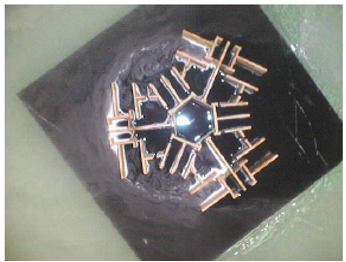
\includegraphics[width=\textwidth]{fig-exemploA}
		\caption{}
		\label{fig-exemploA}
	\end{subfigure}
	\hfill
	\begin{subfigure}[b]{0.45\textwidth}
		\centering
		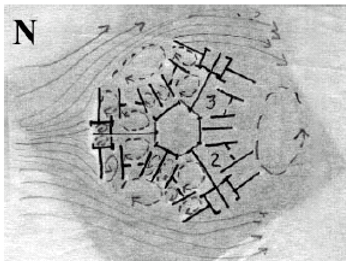
\includegraphics[width=\textwidth]{fig-exemploB}
		\caption{}
		\label{fig-exemploB}
	\end{subfigure}
	\caption*{Fonte: \cite{toledo-pereira:clacs2004}.}
\end{figure}

\begin{grafico}[h]
	\centering
	\caption{Consumo final de energia por fonte no Brasil em 2011}
	\label{graf-exemplo}
	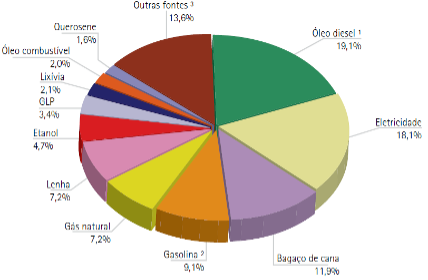
\includegraphics[width=.75\textwidth]{graf-exemplo}	
	\caption*{Fonte: \cite{epe:ben2011}.}
\end{grafico}

As tabelas e os quadros, apesar de possuírem certa semelhança entre si, diferenciam-se não apenas no formato exigido, mas também pelo conteúdo que exibem:

\begin{enumerate}[label=\alph*)]
	\item um quadro apresenta informações ou resultados qualitativos, ou seja, em forma de texto, mesmo que este empregue números;
	\item uma tabela apresenta informações ou resultados quantitativos, ou seja, números tratados estatisticamente.
\end{enumerate}

Quanto ao formato e à apresentação de tabelas e quadros, como se verifica na Tabela~\ref{tbl-exemplo} e no Quadro~\ref{qdr-exemplo}, devem-se observar as seguintes regras~\citep{fibge:nat1993}:

\begin{enumerate}[label=\alph*)]
	\item a moldura das tabelas não deve ser fechada com traços verticais à esquerda e à direita;
	\item deve-se evitar o uso de traços verticais para separar as colunas e de traços horizontais para separar as linhas de uma tabela;
	\item o quadro é um elemento fechado, portanto, deve conter traços horizontais e verticais para separar suas linhas e colunas, além de traços horizontais e verticais para delimitar sua moldura.
\end{enumerate}

\begin{table}[h]
	\centering
	\caption{Exemplo de formatação de uma tabela para a apresentação de resultados}
	\label{tbl-exemplo}
	\begin{tabular}{ccc}
		\hline
		\textbf{Grupos de idade [meses]} & \textbf{Número de indivíduos no grupo} & \textbf{Indivíduos viáveis [\%]} \\
		\hline
		0 -- 10		& 20	& 9,0
\\
		10 -- 15	& 20	& 10,0
\\
		15 -- 20	& 25	& 4,0
\\
		Acima de 20	& 15	& 3,4
\\
		\hline	
	\end{tabular}
	\caption*{Fonte: Produção do próprio autor.}
\end{table}

\begin{quadro}[h]
	\centering
	\caption{Dimensionamento dos elementos de um conversor \textit{boost}}
	\label{qdr-exemplo}
	\begin{tabular}{|p{60mm}|p{60mm}|}
		\hline
		\rowcolor{gray!25}
		\centering \textbf{Elemento ou Grandeza} &  \centering \textbf{Valor ou Modelo}
		\tabularnewline
		\hline
		Tensão de entrada 		& $48 V$
		\\\hline
		Tensão de saída 		& $200 V$
		\\\hline
		Potência de saída 		& $200 W$
		\\\hline
		Frequência de comutação	& $50 kHz$
		\\\hline
		Indutor de entrada 		& $880 \mu H$
	\\\hline
		Capacitor de saída 		& $22 \mu F$
	\\\hline
		Diodo					& $FES8HT$
		\\\hline
		Interruptor				& $IRFP360$	
	\\\hline
	\end{tabular}
	\caption*{Fonte: \cite{menegaz:thesis2005}.}
\end{quadro}

Outros elementos textuais que podem fazer parte do subprojeto de pesquisa são as equações e fórmulas. Para facilitar a leitura, a NBR 15287:2011 exige que as equações sejam destacadas do texto e numeradas com algarismos arábicos entre parênteses, alinhados à margem direita da página, como mostra a Equação~\eqref{eqn-exemplo}. Assim como no caso de figuras, tabelas e quadros, a citação, ou a chamada, de todas as equações ou fórmulas no texto é obrigatória, e sua localização deve acontecer o mais próximo possível do trecho onde são mencionadas pela primeira vez.

\begin{equation}
	\label{eqn-exemplo}
	v_{r}(t) = R \times i(t)
\end{equation}



%%%%%%%%%%%%%%%%%%%%%%%%%%%%%
\section{Objetivos}

Esta seção deve conter, de forma concisa, o objetivo geral e os objetivos específicos do subprojeto, ou seja, as hipóteses que se quer demonstrar, os dispositivos que se quer montar, os compostos que se deseja sintetizar, as ideias que se deseja corroborar ou refutar e etc. Também deve-se dar, de forma concisa, as razões pelas quais se quer atingir estes objetivos.

 

%%%%%%%%%%%%%%%%%%%%%%%%%%%%%
\section{Metodologia}

Deve-se definir, com base na revisão bibliográfica ou em trabalhos preliminares, a metodologia que deverá ser adotada para testar a hipótese formulada e atingir os objetivos estabelecidos. Apresentar o procedimento de trabalho, o material que deverá ser utilizado, o tratamento da informação e o procedimento estatístico, se for o caso. Esta seção deve, entretanto, detalhar os aspectos da metodologia empregada nas atividades especificamente a serem executadas pelo estudante e apresentar sua relação com o projeto de pesquisa ao qual o subprojeto está vinculado.



%%%%%%%%%%%%%%%%%%%%%%%%%%%%%
\section{Plano de Trabalho / Cronograma}

Esta seção deve explicitar as atividades que serão desenvolvidas pelo estudante (Quadro~\ref{qdr-atividades}) e seu cronograma de execução (Quadro~\ref{qdr-cronograma}) para que os objetivos do subprojeto possam ser alcançados, especificando período de início e término. As atividades não devem ser apenas listadas, sendo necessário apresentar uma breve descrição de sua relevância para o subprojeto proposto e a forma de execução.

O cronograma de trabalho de pesquisa deverá organizar a sequência das atividades planejadas. É obrigatório prever, para o mês de fevereiro de 2022, a elaboração, pelo estudante, do relatório parcial da pesquisa, e para o mês de agosto de 2022, a elaboração do relatório final.


\begin{quadro}[h]
	\centering
	\caption{Lista de atividades previstas do subprojeto}
	\label{qdr-atividades}
	\begin{tabular}{|p{145mm}|}
	\hline
	a) Xxxx -- xxxxxxxxx \\
	\hline
	b) Yyyy -- yyyyyyyyy \\
	\hline
	c) Zzzzz -- zzzzzzzz \\
	\hline
	\end{tabular}
	\caption*{Fonte: Produção do próprio autor.}
\end{quadro}

\begin{quadro}[h]
	\centering
	\caption{Cronograma de atividades previstas do subprojeto (set./2021 a ago./2022)}
	\label{qdr-cronograma}
	\begin{tabular}{|p{2.7cm}|l|l|l|l|l|l|l|l|l|l|l|l|}
	\hline
	Atividade & set. & out. & nov. & dez. & jan. & fev. & mar. & abr. & maio & jun. & jul. & ago. \\
	\hline
	a) Xxxx &   &   &   &    &  &   &   &   &   &   &   &  \\
	\hline
	b) Yyyy &   &   &   &   &   &   &    &    &   &   &   &  \\
	\hline
	c) Zzzzz &   &   &   &   &   &   &   &   &    &   &  & \\
	\hline
	\end{tabular}
	\caption*{Fonte: Produção do próprio autor.}
\end{quadro}



%%%%%%%%%%%%%%%%%%%%%%%%%%%%%
\section*{Declaração}

Eu, professor(a) candidato(a) a orientador(a), declaro que o subprojeto de pesquisa aqui proposto é passível de ser realizado ainda que as condições de isolamento social a que ora estamos submetidos se estendam durante toda a vigência do edital PIIC 2021/2022.


%\bibliographystyle{apalike2}
\bibliographystyle{hapalike2-NOand}

\bibliography{biblio}


\end{document}



